\subsection{Dust Attenuation}\label{sec:modelling.dust}
To compare to the galaxy observables at this redshift requires treatment of the simulation data to create mock observations. One of the most important ingredient in generating such mock observations involves modelling the attenuation by dust. It has a major impact on the observed properties of galaxies with almost 30$\%$ of all photons in the Universe having been reprocessed by dust grains at some point in their lifetime \citep{Bernstein2002}. There have been a few studies that have incorporated dust creation and destruction self-consistently into hydrodynamical simulations \citep[\eg][]{Aoyama2017,McKinnon2016a,Gjergo2018,dave_simba:_2019,Graziani2020} and have been successful in prediction of some of the observed properties which eliminate the many post-processing assumptions, but these are compuationally intensive and involve additional subgrid recipes which are poorly understood. A simple alternative is to model the effect of dust based on the properties of the existing stars and gas particles in the simulation.

In this work, for estimating the attenuation by dust, each star particle is treated as a point in space with it's emitted light reaching the observer through the intervening gas particles, with the viewing angle fixed to be along the z-axis. The effect of any star particle along the same line-of-sight (LOS) is ignored. For the purpose of this study we link the metal column density ($\Sigma (x,y)$) integrated along the LOS (z-axis) to the dust optical depth in the V-band (550nm) due to the intervening interstellar medium (ISM) $\tau_{\textrm{ISM,V}}(x,y)$, the same approach as in \cite{Wilkins2017}. This relation can be expressed as
\begin{equation}\label{eq: tau}
\tau_{\textrm{ISM,V}}(x,y) = \kappa_{\textrm{ISM}} \Sigma (x,y)
\end{equation} 
where $\kappa_{\textrm{ISM}}$ is a normalization parameter which we have chosen to match the rest-frame far-UV (1500\AA) luminosity function to the observed UV luminosity function from \cite{Bouwens_2015a} at $z=5$. Thus $\kappa_{\textrm{ISM}}$ acts as a proxy for the properties of dust such as the average grain size, shape, composition as well as the dust-to-metal ratio in the ISM. It is worthwhile noting that dust-to-metal ratios of galaxies are not necessarily constant across redshift, but possibly a function of their evolutionary stage \citep[see][etc]{DeVis2019,Vijayan2019} with the median value decreasing with increasing redshift. Hence this may cause our simple model to overpredict the attenuation of galaxies progressively with redshift. In a companion work we will explore the impact of a range of different modelling approaches.

\begin{figure}
	\centering
	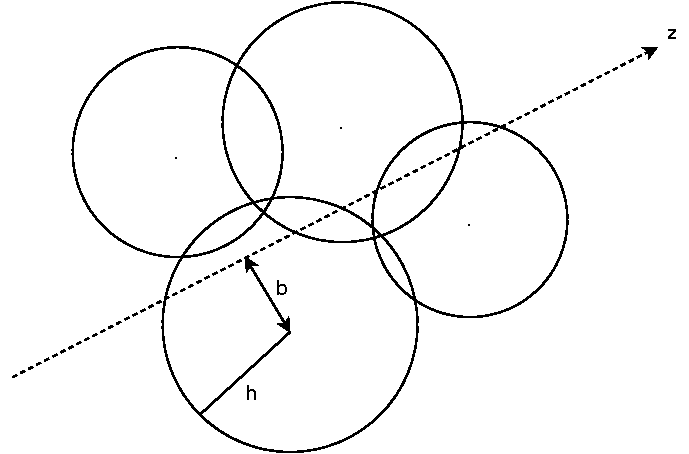
\includegraphics[width=0.4\textwidth]{./figures/sph_ray}
	\caption{Line of sight tracing of the sph density field,  with the circles representative of sph particles. h and b denote the smoothing length of the corresponding gas particle and the impact parameter to the line of sight ray respectively. \label{fig: sph_ray}}
\end{figure}

$\Sigma (x,y)$ is obtained by integrating the density field of particles along the z-axis with the smoothing kernel of the SPH particle. \textsc{Flares} uses the same flavour of SPH used by \textsc{Eagle}, \textsc{Anarchy} \citep[see][for more details]{Schaller2015}. The kernel function can be expressed as follows:
\begin{equation}\label{eq: kernel}
W(r,h) = \dfrac{21}{2\pi\,h^3} 
\begin{cases}
(1-\frac{r}{h})^4 (1+4\frac{r}{h})& \text{if } 0 \leq r\leq h\\
0  & \text{if }r>h
\end{cases}
\end{equation}
where h is the smoothing length of the corresponding particle and r is the distance from the centre of the particle. The smoothed density line integral across a particular particle can be calculated by using the impact parameter, b which is calculated from the centre of the particle (illustrated in Figure~\ref{fig: sph_ray}). Using the impact parameter of every gas particle in front of the selected stellar particle, the LOS metal column density can be calculated as follows:
\begin{equation}\label{eq: Zlos}
\Sigma (x,y) = 2 \sum_i Z_i m_i \int_{0}^{\sqrt{h_i^2-b_i^2}}W(r, h_i)dz\,;\, r^2 = b_i^2 + z^2
\end{equation} 
where the index `i' denote gas particles along the LOS, with Z and m the metallicity and mass of the particle respectively. 
To simplify this calculation, impact parameters can be normalized with the smoothing length, and thus generate pre-computed values of the LOS metal density which can be readily used to compute the density for arbitrary values of smoothing length and impact parameters.

Other than the dust extinction along the LOS, there is an additional component of dust that affects young stellar populations that are still embedded in their birth cloud. Effect of the birth cloud attenuation in our galaxies is a phenomenon that happens below the resolution scale, since stellar clusters form on sub-kpc scales. The birth cloud dust optical depth in the V-band for our model can be expressed in a similar manner to equation \ref{eq: tau} as
\begin{equation}
	\tau_{\textrm{BC,V}}(x,y) = 
	\begin{cases}
	\kappa_{\textrm{BC}} (\textrm{Z}/0.01)\, & \text{t} \leq 10^7\textrm{yr}\\
	0\, & \text{t} > 10^7\textrm{yr}
	\end{cases}
\end{equation}  
where $\kappa_{\textrm{BC}}$ just like $\kappa_{\textrm{ISM}}$, is a normalization factor, while Z is the metallicity of the stellar particle with age less than 10$^7$yr, following the assumption from \cite{Charlot_and_Fall2003} that birth clouds disperse on these timescales. Hence only those young stellar particles are affected by this additional attenuation. With these parameters the optical depth in the V-band is linked to other wavelength using a simple simple power-law relation
\begin{equation}\label{tau_lambda}
	\tau_{\lambda} = (\tau_{\textrm{ISM}} + \tau_{\textrm{BC}}) \times\,(\lambda/550\textrm{nm})^{-1}
\end{equation}
As discussed earlier there are two free parameters in our model, $\kappa_{\textrm{ISM}}$ that links the optical depth in the ISM to the LOS metal surface density and $\kappa_{\textrm{BC}}$ linking the stellar particle metallicity to the optical depth due to the presence of a birth cloud in young stellar populations. The value for these parameters in our model is obtained by first varying $\kappa_{\textrm{BC}}$ within a range of (0.0001, 3.) to get a value for $\kappa_{\textrm{ISM}}$ by fitting the observed UV luminosity function from \cite{Bouwens_2015a} at $z=5$. We choose $\kappa_{\textrm{BC}}$ so as to match observations of the UV-continuum slope ($\beta$) as well as the equivalent-width (EW) relations (OIII doublet and H$_{\beta}$) from \cite{deBarros19_OIIIHbeta} at $z=8$, while the value of $\kappa_{\textrm{ISM}}$ follows by calibrating for the UV LF at $z=5$. We would also like to point out that our selection of $\kappa_{\textrm{BC}}$ is a way to incorporate both of these observations, as a higher value is favoured to get better agreement with the UV-continuum observations while the EW relations prefer a lower value. \chris{is it a pain to run two models, one matching the UVLF, the other the EW observations? perhaps something to keep in mind as I can imagine a referee asking about the parameter dependence} This study uses $\kappa_{\textrm{BC}}=1.25$ and $\kappa_{\textrm{ISM}}=0.0063$ for all the redshifts considered in this study. We would like to remind the reader that this implies no evolution in the dust-to-metal ratio as well as the general properies of the dust grain in galaxies. The parameter search is explained further in Appendix \ref{app:calibration}.

We also show in Appendix \ref{app:extinction_curves} how some of the observables presented in the next sections change on using different extinction curves available from literature.

\chris{Do you resample in time recently formed star particles and highly star forming gas particles? Lots of stuff in Trayfords papers about how this affects emission, as the star formation creates too much mass in too small bursts.}
